\documentclass[letterpaper, 10 pt, conference]{../ieeeconf} 
\IEEEoverridecommandlockouts
\overrideIEEEmargins
\pdfoptionpdfminorversion=4

\usepackage{amsmath}
\usepackage{mathtools}
\usepackage{textcomp}
\usepackage{graphicx}
\usepackage[font=footnotesize]{subcaption}
\usepackage[font=footnotesize]{caption}
\usepackage{hyperref}
\usepackage{amssymb}
\usepackage{booktabs}
\usepackage[normalem]{ulem}
\usepackage{verbatim}
\usepackage[export]{adjustbox}
\usepackage{amsmath}
\usepackage{url}
\usepackage{siunitx}
\usepackage[utf8]{inputenc}
\usepackage[TS1,T1]{fontenc}
\usepackage{array, booktabs}
\usepackage{caption}
\usepackage[cal=cm]{mathalfa}
\usepackage{algorithm}
\usepackage[noend]{algpseudocode}

% Labels in IEEE format
\newcommand{\eref}[1]{(\ref{#1})} % Equation
\newcommand{\sref}[1]{Sec.~\ref{#1}} % Section
\newcommand{\figref}[1]{Fig.~\ref{#1}} % Figure
\newcommand{\tref}[1]{Table~\ref{#1}} % Table
\newcommand{\aref}[1]{Algorithm~\ref{#1}} % Algorithm
\newcommand{\lref}[1]{Line~\ref{#1}} % Line
\renewcommand*\rmdefault{ppl}
\setlength{\textfloatsep}{5pt}

\usepackage{ifthen}
\usepackage[usenames,dvipsnames,table]{xcolor}
\newboolean{include-notes}
\setboolean{include-notes}{true} 
% http://en.wikibooks.org/wiki/LaTeX/Colors
\newcommand{\rhnote}[1]{\ifthenelse{\boolean{include-notes}}%
 {\textcolor{blue}{\textbf{RH: #1}}}{}}
\newcommand{\sanote}[1]{\ifthenelse{\boolean{include-notes}}%
 {\textcolor{green}{\textbf{SAN: #1}}}{}}

\begin{document}

% paper title
\title{6.857 Final Project: Milestone 5}
\author{Sebastiani Aguirre Navarro and Rachel Holladay}
\maketitle

\section{Introduction}
Our goal is to use neural networks to classify whether a particular grasp will succeed on an object.
We utilize the Dexerity Network (DexNet) 2.0 data set~\cite{mahler2017dex}, that has 6.7 million synthetic point clouds with parallel-jaw grasps (a common robot hand type of two parallel fingers) and analytical grasp metrics.
The authors of the data set trained a Grasp Quality Convolutional Neural Network (GQ-CNN), which achieved 85.7\% accuracy on their classification task.
To accomplish the same task, we will be experimenting with new architectures, intput formats, other modifications described in~\sref{sec:questions}.
Through our experimentation we hope to first better understand how these parameters effect learning and to hopefully improve upon the accuracy. 

We will first describe the data set generation process and the features provided in the data set~\sref{sec:data_set}. 
Understanding and processing this data set has become a larger element of our project then previously anticipated. 
We next discuss our results thus far~\sref{sec:results}, which are preliminary. 
We will continue to explore these results, as well as our research questions~\sref{sec:questions}. 


\section{Data Set}
\label{sec:data_set}
We are using the Dex Net 2.0 data set as first presented in~\cite{mahler2017dex}. 
We first briefly summarize their data generation process before describing how we manipulated the data. 

Mahler et al define a generative graphical model defined over the camera pose, object shape and pose, friction coeffient, grasp, depth image and success metric. 
To generate the data set they make i.i.d (independent and identically distributed) samples from their generative graphical model, resulting in 6.7 million data points. 

The data set is defined over 1,500 object meshes that were used in Dex-Net 1.0~\cite{mahler2016dex}, collected from a variety of other data bases and standardized with respect to position.
For each object, they generated 100 parallel jaw grasps via rejection sampling of antipodal pairs and evaluated a grasp metric on each grasp. 
Additionally, each object is paired with a rendered depth image (2.5D point cloud~\footnote{The images are 2D matrics that are referred to as 2.5D in robotics literature because they display depth information.}) from the sampled camera pose. 

The GQ-CNN takes two images as input. The first is the depth image, called the "aligned image", transformed to center and axis align according the grasp point. 
Hence this image captures the scene and grasp in one representation. 
The second image, the "z image" is untransformed and represents the distance from the gripper to the camera.

The data set of 6.7 million data points has 21.1\% positive examples. 
This is unsurprising, since it is much more difficult to find successful grasps, as compared to failed grasps. 

The published Dex-Net 2.0 data set contains both sets of images for each data point in addition to grasp quality metrics and the grasp, represented by a 7-dimensional vector, specifying details of the grasp center, angle, object center and gripper width. 
Our label is given by the robust epsilon quality grasp metric (defined in~\cite{seita2016large}), which is thresholded by the value 0.002 to create binary labels.

From the 6.7 million data points, we create two types of data sets:
\begin{itemize}
    \item \textbf{Unbalanced.} We randomly sample 10,000 data points from our entire set. We expect to sample approximately 20\% positive examples, matching the distribution of the original set.
    \item \textbf{Balanced.} We randomly sample data points until we have 10,000 data points that are 50\% positive examples and 50\% negative examples. 
\end{itemize}
We further discuss the motivation for this distinction in \sref{sec:questions}. 
For all data sets we include all possible features, although some architectures might not leverage all features. 

\section{Results}
\label{sec:results}
\rhnote{give the results from the architectures that we have}

\section{Research Questions}
\label{sec:questions}

\subsection{Input Format}
\rhnote{our input versus what was used in the paper. also that other concatenated thing}

\subsection{Balancing Data Sets}
\rhnote{number of positive versus negative examples. however the 80/20 split might match real world distribution..}

\subsection{Normalization}
\rhnote{they normalized, should we}

\subsection{Architecture Structure}
\rhnote{list a couple different arch's}

\section{Work Distribution}
\rhnote{give basically same thing as before}

\begin{comment}


Each object is paired with 2.5D point clouds, referred to as depth images, which are rendered with a variety of object and camera poses, where the camera intrinsics are known and used to center the depth image in a standardized fashion.
Each image is a black and white 32 by 32 pixel matrix. 

Therefore, we designed a simple Residual Network like the one shown in \figref{fig:network}. 
The idea is to pass the 32x32 depth maps through a ResNet with Batch Normalization to extract 1x8 features from it, and then these features are concatenated to the hand pose features that are passed to a fully connected layer that ouputs the likelihoods of each binary class. 
The training was carried in Keras~\cite{chollet2017keras}, using the RMSProp optimizer during 50 epochs with a batch size of 32 and 10\% of the dataset was used as Test. 
Given that we had a class imbalance of 1858 positive vs 8150 negatives in our datset subset, we assigned weights of 0.8 for positive and 0.2 for negative such that the underrepresented class could influnce training during each gradient descent step. 
This initial architecture did not work so well, however, since the error in the Test set was 81.0\%. 
If we observe the curves for loss and accuracy on Train and Validation during training in \figref{fig:loss} and \figref{fig:accuracy}, we can see that the network is overfitting. 

\begin{figure*}[t!]
    \begin{subfigure}[t]{0.49\textwidth}
        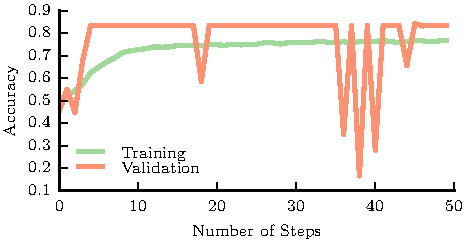
\includegraphics[width=0.99\columnwidth]{figs/accuracy.pdf}
        \caption{Accuracy} \label{fig:accuracy}
        \end{subfigure}
    \begin{subfigure}[t]{0.49\textwidth}
        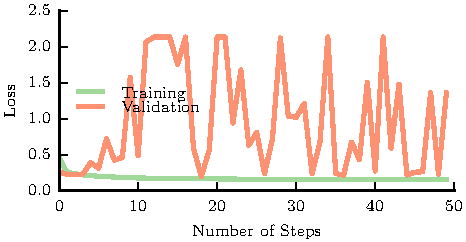
\includegraphics[width=0.99\columnwidth]{figs/loss.pdf}
        \caption{Loss} \label{fig:loss}
    \end{subfigure}
\caption{Initial Loss and Accuracy across the Training and Validation Sets} \label{fig:results}
\end{figure*}

\section{Division of Labor}

Rachel generated the training data from the DexNet data sets and set of the labeling mechanism. 
Sebastiani set up an environment in a AWS with GPUs, coded and trained initial Network In Network, Inception and ResNet based models in Keras/Tensorflow. 

\end{comment}

{\footnotesize
    \bibliographystyle{ieeetr}
\bibliography{../references}}

\end{document}
